\documentclass[../main]{subfiles}

\begin{document}

\clearpage

\setcounter{eqnarray}{0}
\setcounter{equation}{0}
\setcounter{figure}{0}

\part*{第10回}

\subsection{Amp\`ereの法則}
\begin{itembox}[c]{Amp\`ereの法則(微分形)}
\begin{eqnarray}
{\rm rot}{\bf B}=\mu_0{\bf i}
\end{eqnarray}
\end{itembox}
\begin{figure}[htbp]
 \begin{center}
  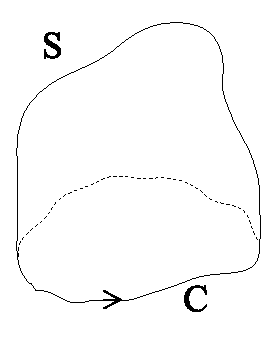
\includegraphics[width=30mm]{9.1.eps}
 \end{center}
 \caption{}
 \label{fig:one}
\end{figure}
Amp\`ereの法則の積分形を導出したい. \\
$C$上に沿って右ねじを巻いたときに進む方向に裏$\to$表を定める.(面積の正負を定める.)
有向ループをふちにもつ任意の曲面$S$にわたる式(1)の面積分を考える.
\begin{eqnarray*}
\int_{S} {\rm rot}{\bf B} \cdot {\bf dS} = \mu_0 \int_{S} &=& \mu_0(\mbox{Sを貫く全電流}) \\
&=& \mu_0(\mbox{Cを貫く全電流})
\end{eqnarray*}
またStokesの定理より,
\begin{eqnarray*}
\int_{S} {\rm rot}{\bf B} \cdot {\bf dS} = \int_{C} {\bf B} \cdot {\bf dl}
\end{eqnarray*}
{\bf 注} \\
\begin{figure}[htbp]
 \begin{center}
  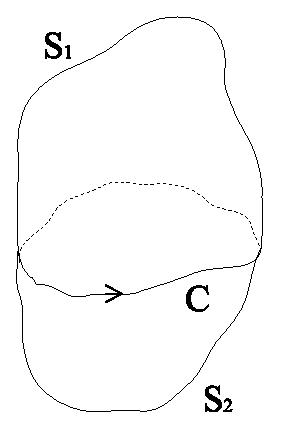
\includegraphics[width=30mm]{9.2.eps}
 \end{center}
 \caption{}
 \label{fig:two}
\end{figure}
\begin{eqnarray*}
\int_{S_1} {\bf i} \cdot {\bf dS} = \int_{S_2} {\bf i} \cdot {\bf dS} \\
\int_{S_1} {\bf i} \cdot {\bf dS} - \int_{S_2} {\bf i} \cdot {\bf dS} = \int_{V} {\rm div}{\bf i}dV = 0
\end{eqnarray*}
\begin{itembox}[c]{Amp\`ereの法則(積分形)}
\begin{eqnarray}
\int_{C} {\bf B} \cdot {\bf dl} = \mu_0(\mbox{Cを貫く全電流})
\end{eqnarray}
\end{itembox}

\begin{figure}[htbp]
 \begin{center}
  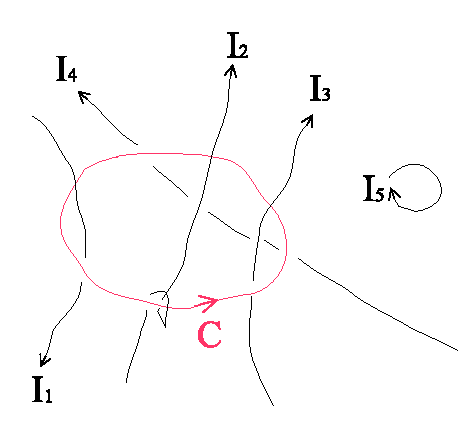
\includegraphics[width=50mm]{9.3.eps}
 \end{center}
 \caption{}
 \label{fig:three}
\end{figure}
{\bf 例} \\
図3では,
\begin{eqnarray*}
\mu_0(\mbox{Cを貫く全電流}) = \mu_0(-{\rm I_1}+2{\rm I_2}+{\rm I_3})
\end{eqnarray*}
{\bf 例1:円電流} \\
\begin{eqnarray*}
B \cdot 2 \pi r = \mu_0 {\rm I} \\
B = \frac{\mu_0{\rm I}}{2 \pi r}
\end{eqnarray*}
{\bf 例2:ソレノイド} \\
\begin{figure}[htbp]
 \begin{center}
  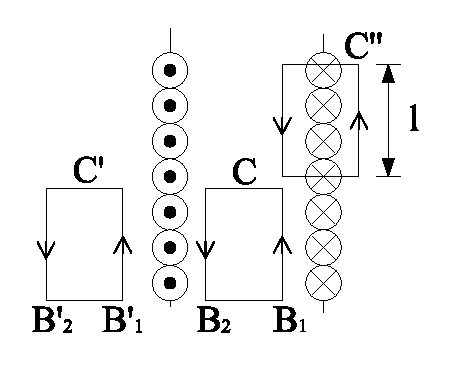
\includegraphics[width=50mm]{9.4.eps}
 \end{center}
 \caption{}
 \label{fig:four}
\end{figure}
\begin{eqnarray*}
C': lB_1'-lB_2'=\mu_0 \cdot 0 \\
B_1'=B_2'=B'
\end{eqnarray*}
したがってソレノイドの外部で磁束密度は一様である. \\
同様に
\begin{eqnarray*}
C: lB_1-lB_2=\mu_0 \cdot 0 \\
B_1=B_2=B
\end{eqnarray*}
したがってソレノイドの内部でも磁束密度は一様である. \\
\begin{eqnarray*}
C'':lB'-lB=-\mu_0 l n {\rm I} \\
\end{eqnarray*}
$B=\mu_0n{\rm I}$であることは以前導いたから,$B'=0$となる.つまりソレノイドの外部では磁束密度は{\bf 0}である.

\subsection{ループ電流と等価磁気双極子層}
\begin{figure}[htbp]
 \begin{center}
  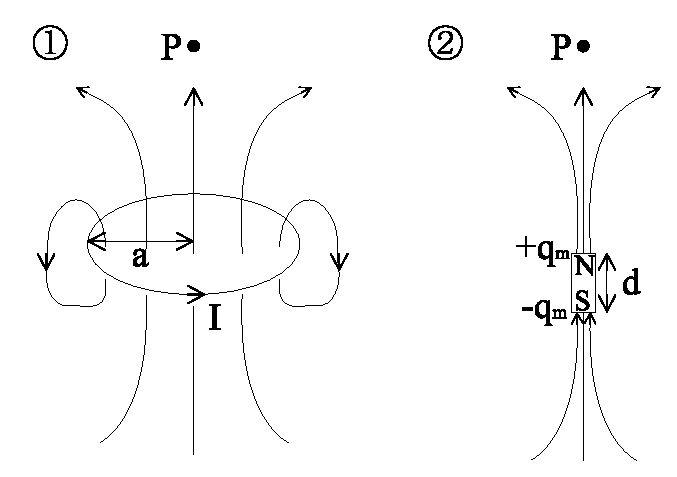
\includegraphics[width=80mm]{9.5.eps}
 \end{center}
 \caption{}
 \label{fig:five}
\end{figure}
仮想的磁荷$\pm q_m [Wb]=[JA^{-1}]$を考えることで,円電流によって生じる磁場と類似したCoulomb的磁場をつくることができる.その磁束密度の大きさは
$|{\bf B}|=\frac{q_m}{4 \pi r^2}$ \\
実はこの2つの磁場は,$a \to 0,I \to \infty , q_m \to \infty ,d \to 0 $の極限で一致する.またこのとき,$\mu_0 \pi a^2 {\rm I}$と$q_md$は同じ極限値$m$をとる. \\
図の点$P$で${\bf B}=(0,0,B_z)$とすると, \\
$\textcircled{\scriptsize 1}$ \\
$a \to 0,I \to \infty$の極限で
\begin{eqnarray*}
B_z = \frac{\mu_0 {\rm I} a^2}{2(z^2+a^2)^{\frac{3}{2}}} \to \frac{m}{2 \pi z^3}
\end{eqnarray*}
$\textcircled{\scriptsize 2}$ \\
\begin{eqnarray*}
B_z = \frac{q_m}{4 \pi} \left( \frac{1}{(z-\frac{d}{2})^2} - \frac{1}{(z+\frac{d}{2})^2} \right)
\end{eqnarray*}
$f(z)=\frac{1}{z^2}$ とすると
\begin{eqnarray*}
B_z &=& \frac{q_m}{4 \pi} \left( f(z-\frac{d}{2})-f(z+\frac{d}{2}) \right) \\
&=& -\frac{q_m d}{4 \pi } \left( \frac{ f(z+\frac{d}{2})-f(z-\frac{d}{2}) }{d} \right)
\end{eqnarray*}
$q_m \to \infty ,d \to 0$の極限で
\begin{eqnarray*}
B_z \to -\frac{m d}{4 \pi} f'(z) = \frac{m}{2 \pi z^3}
\end{eqnarray*}
確かに一致する. \\
一般に,ループ$C$に沿う電流による${\bf B}$は,Cを境界にもつ磁気双極子の層をなす${\bf B}$と等しい.これを,等価磁気双極子層という.

\subsection{Lorentz力}
\begin{itembox}[c]{Lorentz力}
\begin{eqnarray}
{\bf F} = q ({\bf E} + {\bf v} \times {\bf B})
\end{eqnarray}
\end{itembox}
両辺に速度${\bf v}$を掛けると
\begin{eqnarray*}
{\bf F}\cdot{\bf v} = q ( {\bf E}\cdot{\bf v} + {\bf 0} )
\end{eqnarray*}
つまり${\bf B}$は仕事をしないことが分かる. \\
\\
電流素片に働く力 \\
\begin{figure}[htbp]
 \begin{center}
  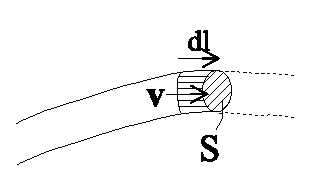
\includegraphics[width=50mm]{9.6.eps}
 \end{center}
 \caption{}
 \label{fig:six}
\end{figure}
電流素片がもつ電荷$dq=\rho S|{\bf dl}|$ \\
\begin{eqnarray*}
{\bf dF}&=&dq{\bf v} \times {\bf B} \\
&=&\rho S |{\bf dl}| {\bf v} \times {\bf B} \\
&=&\rho S |{\bf v}| {\bf dl}  \times {\bf B}
\end{eqnarray*}
ここで$S |{\bf v}| {\bf dl}$の単位に注目すると, \\
\begin{eqnarray*}
Cm^{-3} \cdot m^2 \cdot ms^{-1} = A
\end{eqnarray*}
したがって$S |{\bf v}| {\bf dl}$は電流{\rm I}を表す.
\begin{eqnarray*}
{\bf dF} ={\rm I} {\bf dl}  \times {\bf B}
\end{eqnarray*}
電流,磁場,Lorentz力の方向の関係は,必要とあらば左手で確認できる.(Flemingの左手の法則)
さて今ここで電流の単位アンペアを定義する. \\
そのために,平行に並んだ電線を同じ方向に流れる電流を考える. \\
線電流${\rm I_1}$ が距離d離れた場所に作り出す磁場は,$B_1=\frac{\mu_0 {\rm I_1}}{2 \pi d}$である.そしてその磁場によって${\rm I_2}$の長さ$\Delta l$の部分が受けるLorentz力の大きさは,$F={\rm I_2} \Delta l B_1=\Delta l \frac{\mu_0 {\rm I_1}{\rm I_2}}{2 \pi d}$である. \\
この状態で${\rm I_1}={\rm I_2},d=1{\rm m}$としたときに電線1mあたりに及ぼしあうLorentz力が$2 \times 10^{-7} {\rm N}$となるときの電流の値を$1{\rm A}$と定義する. \\
するとそこから$\frac{\mu_0}{4 \pi}=10^{-7} {\rm NA^{-2}}$が定まることになる. \\
\\
{\bf 例:一様な磁場中の荷電粒子の運動} \\
運動方程式は
\begin{eqnarray*}
m\frac{d{\bf v}}{dt}=q{\bf v} \times {\bf B}
\end{eqnarray*}
だから,
\begin{eqnarray*}
m\frac{dv_x}{dt}&=&qv_yB \\
m\frac{dv_y}{dt}&=&-qv_xB \\
m\frac{dv_z}{dt}&=&0
\end{eqnarray*}
したがって$v_z=\mbox{一定}$であり,x,y成分については,サイクロトロン振動数$\omega=\frac{qB}{m}$とすることにより,
\begin{eqnarray*}
\ddot{v}_x=-\omega^2v_x \\
\ddot{v}_y=-\omega^2v_y
\end{eqnarray*}
\end{document}

